This section discuss the pain maps, and how they are processed before using them as input in deep learning models. Furthermore, the multiple pain maps representations are described, whereafter the complexity of the pain maps was investigated by using linear regressions. Finally, the deep learning architectures were presented.

\subsection*{\textbf{Pain maps}}
Data used in this study were collected from an on-going clinical trial (FOXH) which is conducted in collaboration with Danish and Australian universities. The pain maps were drawn by individuals with PFP syndrome through the use of an application, Navigate Pain, in a clinical setting. \newline
\noindent
Navigate Pain is a software application that is used to visualise the location, morphology and spatial distribution of pain from individuals to healthcare personnel. The application permits individuals to draw their pain with different colors and line thickness onto a body outline, an example is shown in fig. \ref{fig:twoPainmaps}. Navigate Pain android was developed at Aalborg University.\citep{Solutions2015}

\begin{figure}[H]
\centering
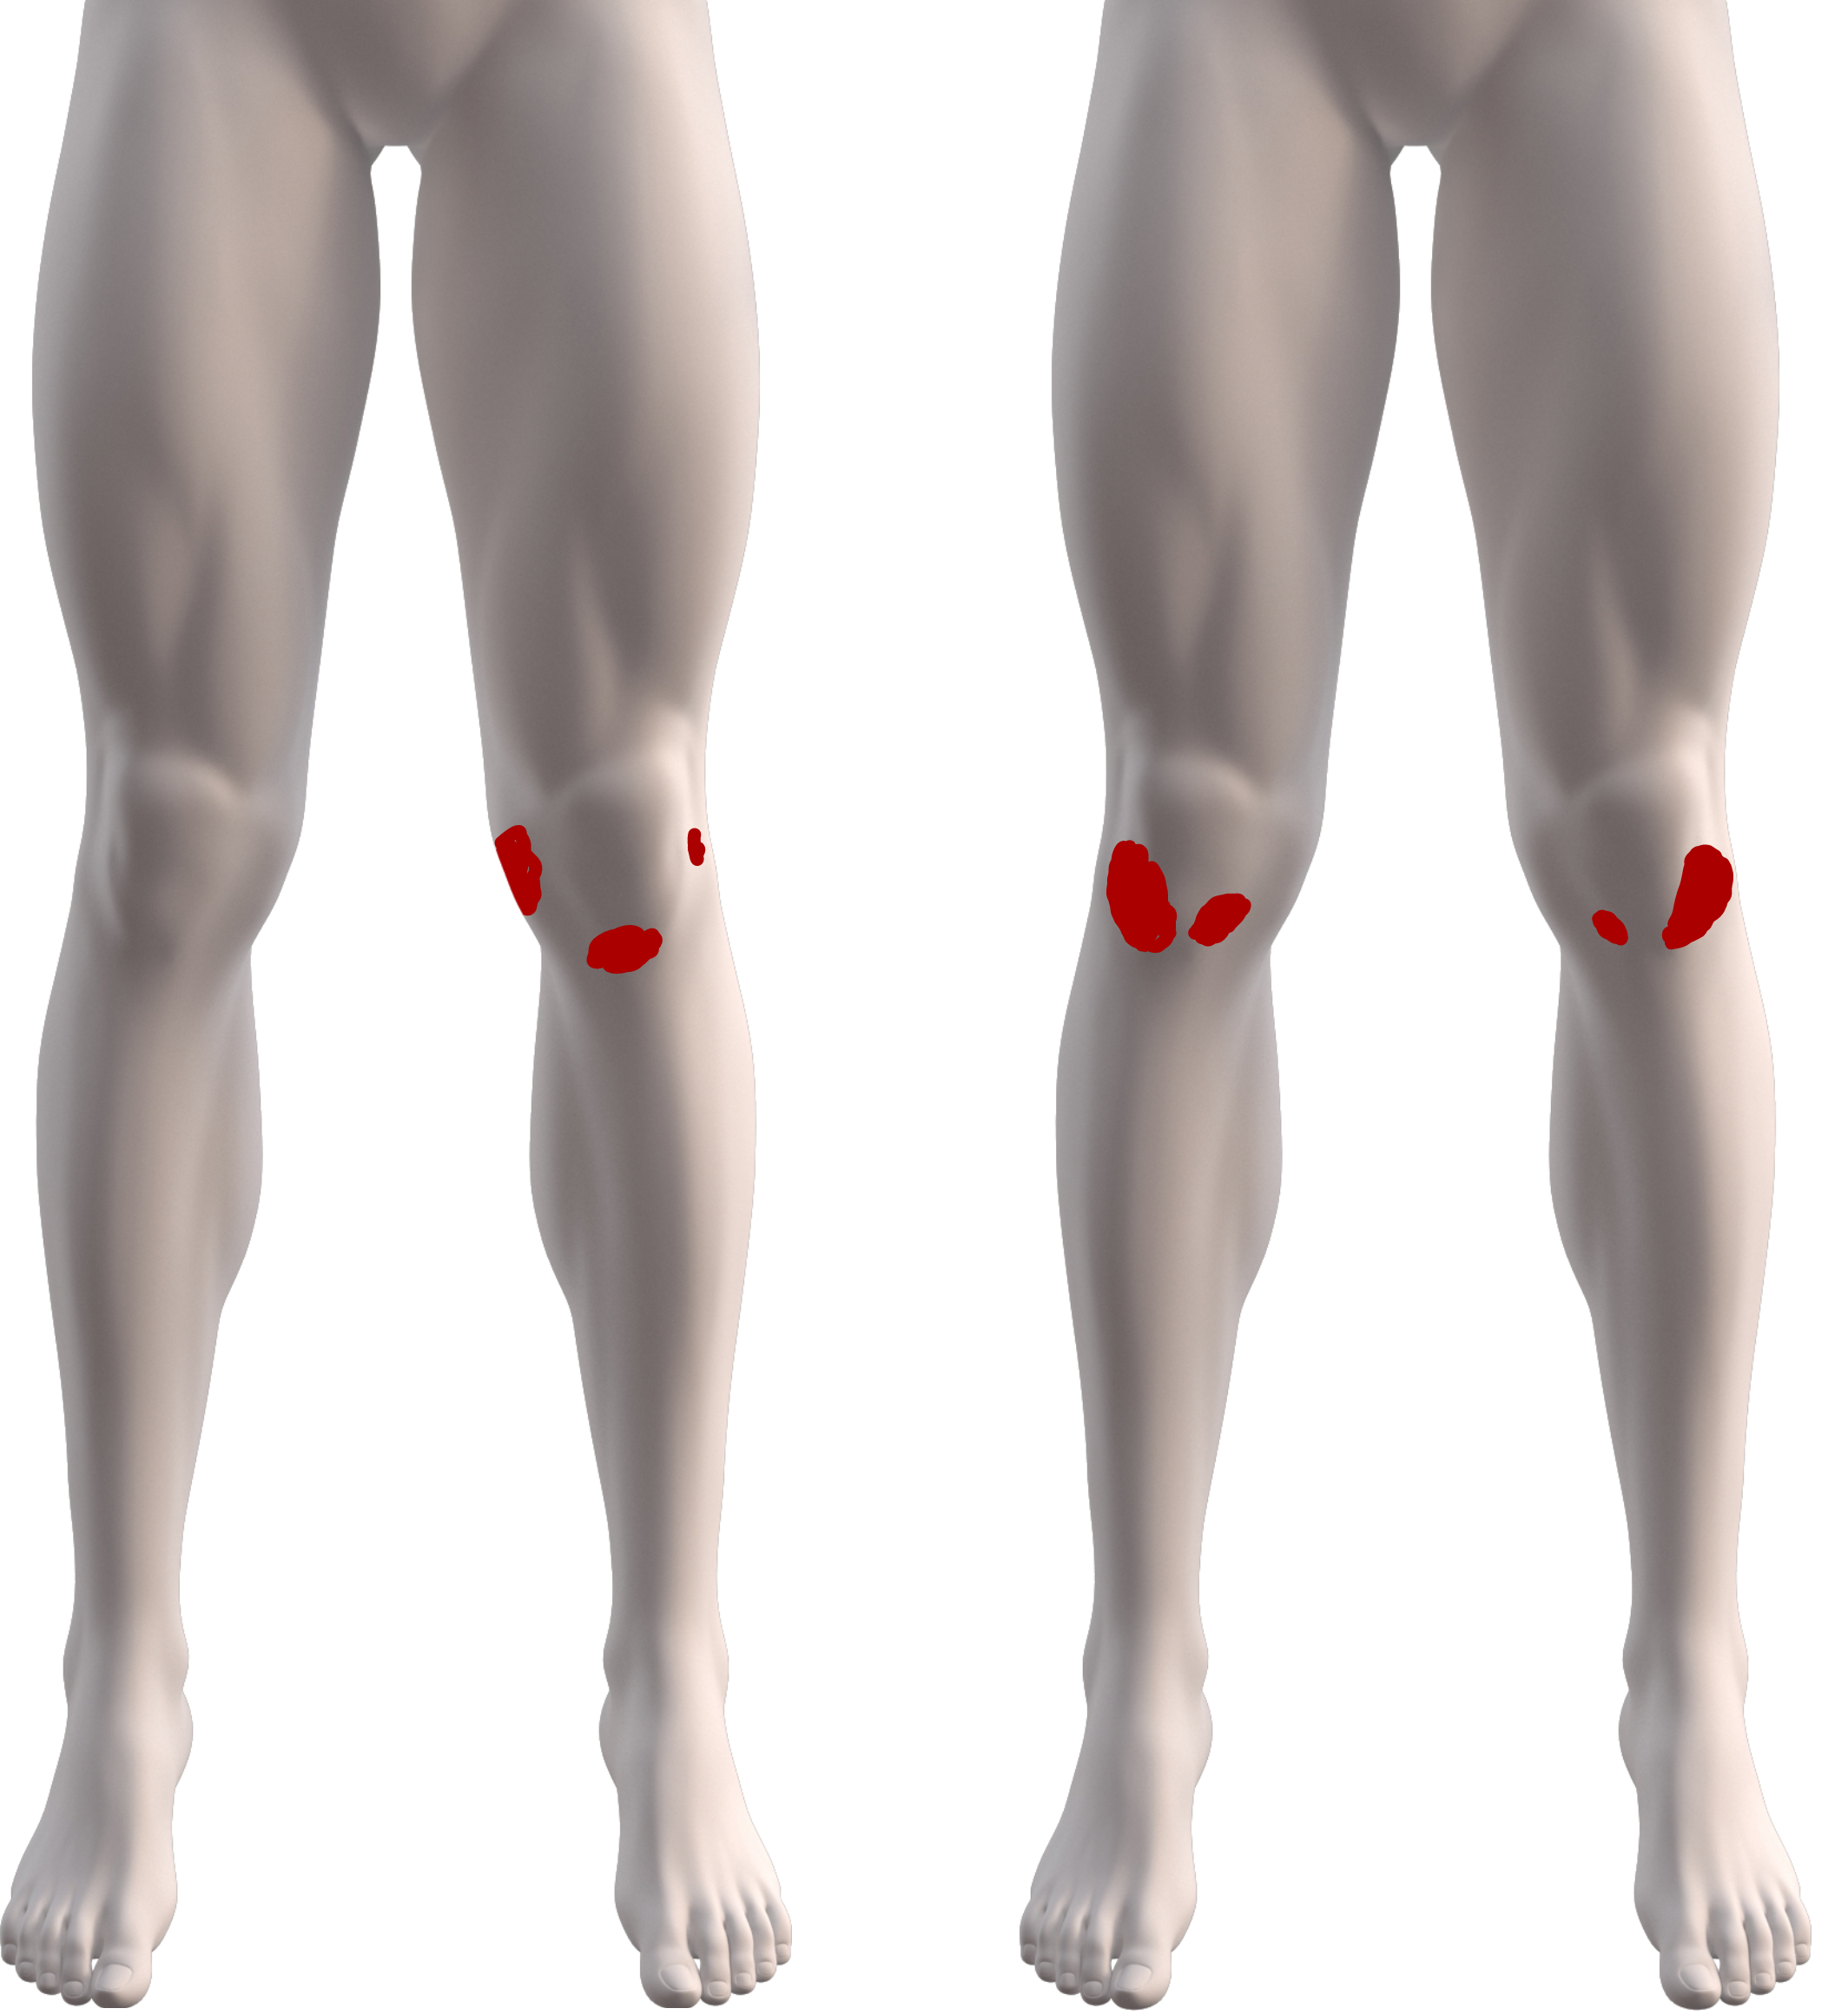
\includegraphics[width=0.3\textwidth]{Figures/twoPainmaps}
\caption{Pain maps from individuals with uni- and bilateral PFP. The red markings indicate the area of pain perceived by the individuals.}
\label{fig:twoPainmaps}
\end{figure}

\noindent
The total number of pain maps available was 217, but only 205 pain maps with associated pain duration, and 197 pain maps with associated pain intensity was available. The gender was included as an input, because females may report a more intense and frequent pain than males. 


\subsection*{\textbf{Preprocessing}}
The pain maps were processed in MatLab version R2017b, where the images were resized to a pixelsize on $252 \times 118$, since they were collected at different resolutions (screen sizes) and cropped to only include the knees. To create more pain maps is a split body approach used, where pain maps are divided into two knees. Furthermore, pain was mirrored to represent pain on right knees to minimize the variance in the images. By using split body approach it was assumable that the pain duration and pain intensity were identical for both knees if PFP was bilateral. The total number of pain maps with gender and pain duration was 333, and pain maps with gender and pain intensity was 319, of which 15\% was used as test data, and therefore not used to optimize and train the models. \newline
\noindent
The models should classify pain maps according to pain duration or pain intensity divided into intervals. These intervals were created based on the extremes, which were 0 to 12 months and 36 to 300 months for pain duration, and 0 to 4 and 8 to 10 for pain intensity. It was chosen to divide into extremes, since it was assumed that
if the models predicted badly with the extremes, the models would not have a higher predictive value with multiple classifications of the outputs.

\subsection*{\textbf{Morphology-representation}}
The original pain maps reflect the morphology of the pain, and do not require further processing than converting the pain maps to a matrix including gender and the output, pain duration or pain intensity. As a result of using the extremes for classifying the number of pain maps decrease to 236 for pain duration, and 196 for pain intensity.

\subsection*{\textbf{Pain location}} 
The knee is divided into regions based on the underlying anatomical structures, which may have a correlation to pain duration or pain intensity.
The locations are divided into 10 regions, which are inspired by Photographic Knee Pain Map (PKPM). The divisions are designed to categorise location of knee pain for diagnostic and research purposes.\citep{Elson2010} The knee regions are illustrated in fig. \ref{fig:atlas}.

\begin{figure} [H] 
\centering
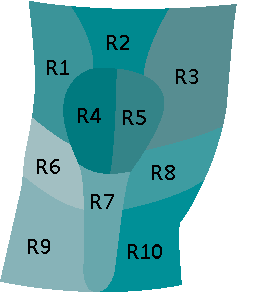
\includegraphics[width=0.22\textwidth]{Figures/atlas}
\caption{The regions of the right knee (R1-R10).}
\label{fig:atlas}
\end{figure}

\noindent 
There are ten regions, where region 1 and 3 represent the superior lateral and superior medial areas for patella. Region 2 refers to quadriceps tendon. The patella is divided into lateral and medial regions, which are region 4 and 5. Region 6 and 8 are lateral and medial joint line areas. Patella tendon is region 7 and the two last regions, 9 and 10, are tibia lateral and medial.\citep{Elson2010}

\subsection*{\textbf{Location-representation}} 
To investigate whether the location alone have a correlation to the outputs, a simplified representation of the pain maps was created. The location of the pain was reflected by the use of the defined knee regions (fig. \ref{fig:atlas}), where each region represented a value of 0 (not active) or 1 (active) in a vector.  The values were defined by using a threshold to determine whether a region was considered active in relation the amount of pain. A threshold was required to increase the confidence of an active pain region by avoiding minimal contributions e.g. small pain areas in the associated regions. Simultaneously the threshold should not be too large so that pain areas was excluded. The threshold was decided based on an analysis on five random pain maps, where threshold values of 0, 5, 10 and 15\% was compared. The threshold represent which minimal percentage of pain should be present in a specific region before it is considered active. Based on the analysis a 5\% threshold was chosen. As a result of using the extremes for classification, and adding the threshold value the number of pain maps with pain duration decrease to 223, and number of pain maps with pain intensity decrease to 186.  

\subsection*{\textbf{Combined-representation}} 
A combination of morphology and location of the pain is created based on components from morphology- and location-representations. The original pain maps are superimposed on the regions, which result in pain pixels reflecting the location with a number from 1 to 10. Before using the representation as input, one-hot encoding approach was used, which made it possible to separate categorical data into binary data \citep{Harris2012}. This means that the 10 values do not have a correlation when analysed in the deep learning model. The number of pain maps with pain duration was 331, and number of pain maps with pain intensity was 317. The number of pain maps increased according to the location-representation, because no threshold was applied in this data-representation. By classifying according to the extremes, the number of pain maps decrease to 234 for pain duration, and 194 for pain intensity.

\subsection*{\textbf{Nonlinearity in pain maps}} 
Given that PFP is subjective and multifactorial it is unlikely that the pain maps and pain duration or pain intensity are linearly correlated. In order to determine if there was a linear relationship, linear regressions were done on simple features reflecting the size of the pain and number of active pain regions. The linear regressions were made in MatLab, and composed a correlation between number of pain pixels and pain duration, number of pain pixels and pain intensity, number of active pain regions and pain duration, and number of active pain regions and pain intensity.

\begin{figure*} [t!]
%\begin{tcolorbox}[colframe=black!30!black, colback=white]
\centering
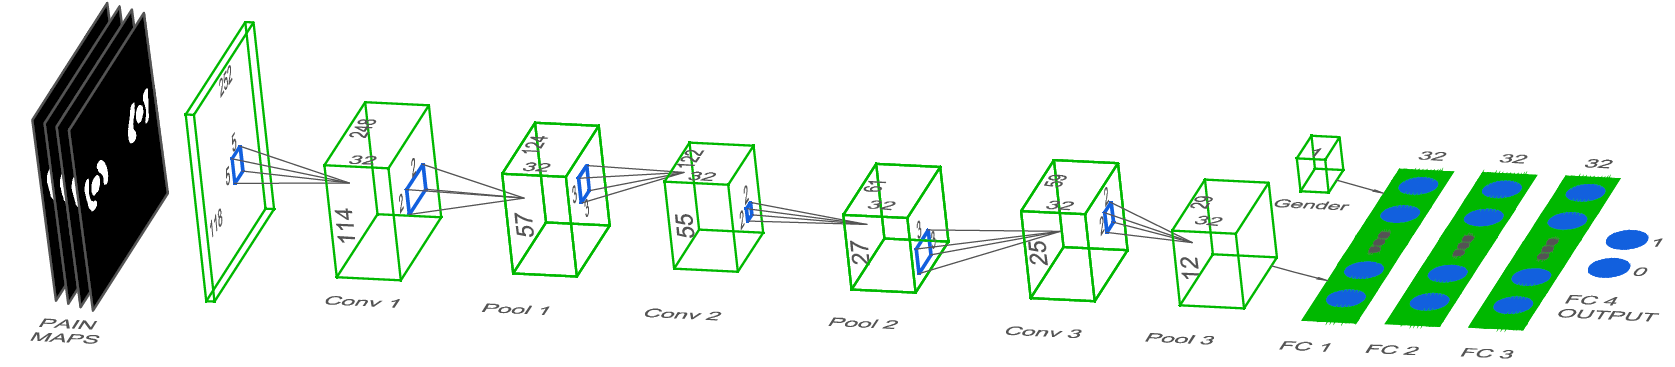
\includegraphics[width=1\textwidth]{Figures/models}
\caption{The architecture of the deep learning models including the morphology-representation consist of three convolutional, three max pooling, and four fully connected layers.}
\label{fig:models}
%\end{tcolorbox}
\end{figure*}

\subsection*{\textbf{Architecture of the deep learning models}}
Deep learning models were developed on a computer with 4x ‘‘Intel® Core™ i7‘‘ CPUs and one single GPU of type "Geforce GTX 970M", using the programming language Python v3.6.3. Libraries used was Keras with a TensorFlow backend. \newline
\noindent
Multiple deep learning models suitable to the three data representation were created. The models used supervised learning, which is defined as a network learning to classify a given input corresponding to a specific output \citep{Goodfellow2016}. The models were designed differently according to its pain maps-representations. The architecture of the models, before  optimization, including the morphology-representation is illustrated on fig. \ref{fig:models}. These models consisted of  three convolutional layers, to which a max pooling layer was designed after each convolutional layer, and ends with four fully connected layers, whereas gender was implemented. The models including the location-representation only use the four fully connected layers of the architecture shown in fig. \ref{fig:models}. The last models using the combined-representation were design similar to the fig. \ref{fig:models}, only with a difference according to the input image, which in this case included images with 10 layers. The models classified the input, pain maps and gender, in relation to the determined outputs, pain duration or pain intensity.

\subsubsection*{\textbf{The convolutional layers}}
Convolutional Neural Networks (CNNs) is a type of special neural network for processing data with a grid-like topology \citep{Goodfellow2016}. CNNs were used to the morphology- and combined-representation because of its capability to perform highly according to image classification. The purpose of the convolutional layer was to recognize the features in the input by taking the image and scan it, then split it up into the feature maps.\citep{Goodfellow2016,LeCun1998} The architecture of the first convolutional layer consisted of a kernel size on $5 \times 5$, and 32 filters. The two following convolutional layers consisted of kernel sizes on $3 \times 3$, and 32 filters. 

\subsubsection*{\textbf{ReLU activation function}}
The activation function chosen for the hidden nodes in all three models were Rectified Linear Unit (ReLu), which transforms the linear output to nonlinear function by making all negative values zero. ReLu function still remains nearly linear, which means it can easily be optimized with gradient descent based methods \citep{Goodfellow2016}. In modern neural networks, ReLU is recommended to use as a default activation function and could be defined as $g(x) = max\{0, x\}$. 

\subsubsection*{\textbf{Max pooling layers}}
For the models containing convolutional layers, the convolution layers are followed by max pooling layers, which is a typical structure of a convolutional network \citep{Goodfellow2016, LeCun2015}.
Max pooling layers are used to reduce the size of the dataset, while maintaining features from the feature map. Given a reduction in the data, the computation speed may increase.\citep{Goodfellow2016,LeCun1998} 
Max pooling layers are defined after each convolutional layer, to which all have a kernel size of $2 \times 2$ with a stride of 2. From the kernel window the highest of the 4 values is extracted to next layer, and used further through the network. 

\subsubsection*{\textbf{Fully connected layer and output layer}}
The models consist of four fully connected layers, whereas the 32 feature maps from the previous layer were flattened, and the notation for gender was included in the end of the string, which was used as input in the first fully connected layer with 32 nodes. Additionally, the second and third layers consisted of 32 nodes. The fourth fully connected layer, which also was the output layer, includes a sigmoid activation function. 
This function operates with a single output, that saturates when its input is either extremely negative or extremely positive \citep{Goodfellow2016}. It refers to the output corresponded to the number of classification intervals, pain duration below 12 month, and above 36 month, or pain intensity below 4, and above 8 on VAS. 


\subsubsection*{\textbf{Dropout algorithm}}
A dropout algorithm was implemented for the models in the last three hidden fully-connected layers to reduce overfitting while training. The algorithm works by randomly drop a specified faction of the nodes in the given layer, to which the nodes that drop changes during training \citep{Srivastava2014}.  Dropout reduce the nodes’ ability for co-adaptation, where multiple nodes compute the same features. For the three models the dropout fraction was set to 0.5 (50\%) based on a previous study by \citeauthor{Srivastava2014} \citep{Srivastava2014}, which considered 0.5 as optimal for a multiple range of networks.   

\subsubsection*{\textbf{Back-propagation algorithm}}
Back-propagation is a learning process where the weights of the models are adjusted in order to reduce the error calculated between the predicted output, and the correct output.\citep{Duda2000} Back-propagation use a method called gradient descents, which computed gradients from the output to the input, in order to minimize the overall output error as much as possible during the learning stage. 
After each pass of a minibatch, the inputs and weights were multiplied of separate node summed with additional coefficient called bias.\citep{LeCun1998, Hameed2016}
Afterwards, a loss was calculated based on a loss function for every input that passed through the network to make the adjustments on the parameters to reduce the loss. As training progressed, the loss should decrease as a result of the parameter adjustments, and improve the performance of the neural network.\citep{Goodfellow2016, LeCun2015, Duda2000}. This learning process continued until optimal parameters with minimum error was reached.\citep{Hameed2016}

\subsection*{\textbf{Training}}
For training the models, a supervised learning approach was used, to which six models were trained, one for each pain map representation, and for each type of classification. 
This process was further combined with a structured grid search on the hyperparameters to help set the initial parameters for the models. These hyperparameters referrers to learning rate, kernel initializer, number of filters and nodes, and number of epochs with different batch sizes. Accuracy was used to determine the improvement of performance when testing the multiple parameters.
Further manual optimization was performed by evaluating the development in loss, and accuracy during training, and the general performance estimated from an accuracy, sensitivity and specificity. After optimization, the models were trained anew using all of the training data, using the optimal hyperparameters from training and tested with a separate test subset.
 

%\begin{figure*} [b!]
%\begin{tcolorbox}[colframe=black!30!black, colback=white]
%\centering
%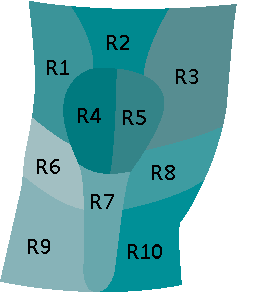
\includegraphics[width=0.2\textwidth]{Figures/atlas}
%\caption{SÅDAN LAVER VI EN BOXER MED ET BILLED}
%\label{fig:atlas1}
%\end{tcolorbox}
%\end{figure*}



%\begin{figure*} [b!]
%\begin{tcolorbox}[colframe=black!30!black, colback=white]
%  \begin{subfigure}[b]{0.45\textwidth}
%    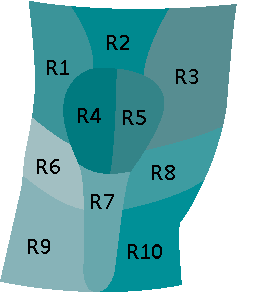
\includegraphics[width=\textwidth]{Figures/atlas}
%    \caption{FUCK JA}
%    \label{fig:f11}
%  \end{subfigure}
%  \hfill
%  \begin{subfigure}[b]{0.45\textwidth}
%    \includegraphics[width=\textwidth]{Figures/twopainmaps}
%    \caption{FUCK NEJ}
%    \label{fig:f22}
%  \end{subfigure}
%  \caption{SÅDAN SÆTTER VI TO BILLEDER I EN}
%\end{tcolorbox}
%\end{figure*}